\documentclass{article}

\usepackage{float,algorithm,graphicx,hyperref,amsmath,amsfonts,verbatim,tikz}
\usepackage[noend]{algpseudocode}
\usetikzlibrary{positioning}

\title{Lab 7 - Neural Networks I}
\author{Kyle Swanson}
\date{January 22, 2018}

\tikzset{%
  every neuron/.style={
    circle,
    draw,
    minimum size=1cm
  },
  neuron missing/.style={
    draw=none, 
    scale=4,
    text height=0.333cm,
    execute at begin node=\color{black}$\vdots$
  },
}

\setcounter{section}{-1}

\begin{document}

\maketitle

\section{Introduction}

\subsection{Lab Overview}

This week we're learning about neural networks, which are the state-of-the-art in machine learning. Deep neural networks in particular have extraordinary computation power and can learn to solve problems and perform tasks that even humans struggle with.

Thanks to the extreme popularity of neural networks recently, there are several excellent libraries (mostly written in Python) which make building deep neural networks easy. We'll be using one of them (keras) in Lab 9. However, I think it's a valuable (and fun!) experience to build a neural network from scratch using only the mathematical operations provided by Python and numpy. My hope is that building a neural network from scratch will give you a better understanding of how neural networks really work on the inside so that you understand what keras and the other neural network libraries are doing behind the scenes.

Building a neural network from scratch takes some work, so I've split it into two labs, Lab 7 (today) and Lab 8 (tomorrow). In these labs, we're going to be building a network with only a single hidden layer (a ``shallow" neural network). In this lab (Lab 7), we're going to be building the prediction part of the network, which will take the input data, pass it through the network, compute the output probabilities, and make a prediction based on the output probabilities. In tomorrow's lab (Lab 8), we'll be implementing the learning portion of the network, which involves using the backpropagation algorithm and gradient descent to update the weights of the network. Once the network is complete at the end of Lab 8, we'll test it on a simple data set and we'll examine the decision boundaries it draws when the network uses different numbers of neurons in its single hidden layer.

\subsection{Single Layer Neural Network}

\subsubsection{Neural Networks Overview}

% https://tex.stackexchange.com/questions/153957/drawing-neural-network-with-tikz
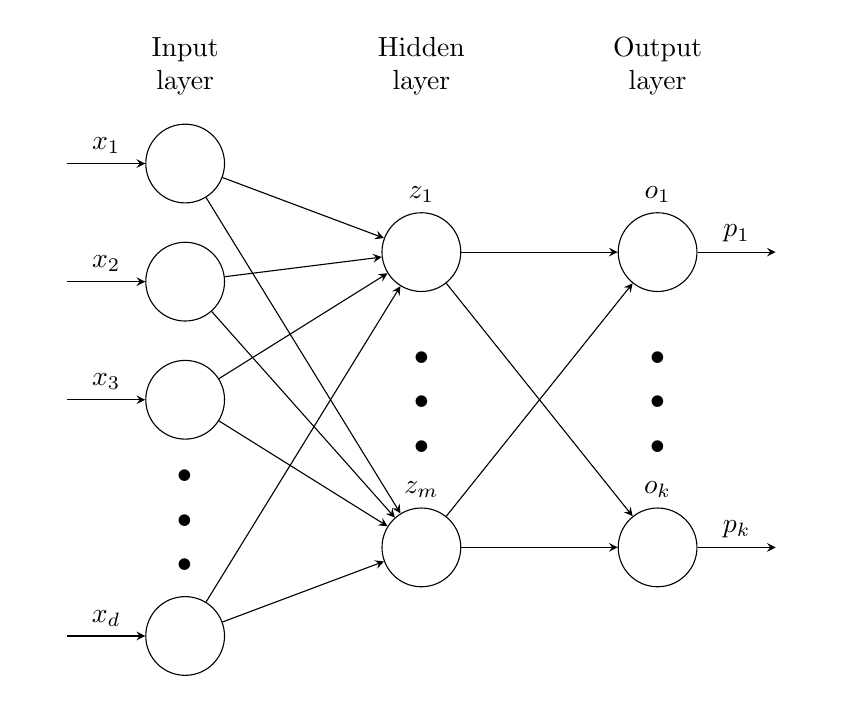
\begin{tikzpicture}[x=1.5cm, y=1.5cm, >=stealth]

\foreach \m/\l [count=\y] in {1,2,3,missing,4}
  \node [every neuron/.try, neuron \m/.try] (input-\m) at (0,2.5-\y) {};

\foreach \m [count=\y] in {1,missing,2}
  \node [every neuron/.try, neuron \m/.try ] (hidden-\m) at (2,2-\y*1.25) {};

\foreach \m [count=\y] in {1,missing,2}
  \node [every neuron/.try, neuron \m/.try ] (output-\m) at (4,2-\y*1.25) {};

\foreach \l [count=\i] in {1,2,3,d}
  \draw [<-] (input-\i) -- ++(-1,0)
    node [above, midway] {$x_\l$};

\foreach \l [count=\i] in {1,m}
  \node [above] at (hidden-\i.north) {$z_\l$};
  
\foreach \l [count=\i] in {1,k}
  \node [above] at (output-\i.north) {$o_\l$};

\foreach \l [count=\i] in {1,k}
  \draw [->] (output-\i) -- ++(1,0)
    node [above, midway] {$p_\l$};

\foreach \i in {1,...,4}
  \foreach \j in {1,...,2}
    \draw [->] (input-\i) -- (hidden-\j);

\foreach \i in {1,...,2}
  \foreach \j in {1,...,2}
    \draw [->] (hidden-\i) -- (output-\j);

\foreach \l [count=\x from 0] in {Input, Hidden, Output}
  \node [align=center, above] at (\x*2,2) {\l \\ layer};

\end{tikzpicture}

As a reminder, above is a diagram of a single layer neural network. The first layer is the input layer. If our input data points are $d$-dimensional, then there will be $d$ input units. The middle layer is the hidden layer, which consists of $m$ neurons ($m$ is a number that we get to choose). The final layer is the output layer, which consists of $k$ neurons where $k$ is the number of classes that we're trying to choose between. For instance, if we're trying to predict whether an image shows a car, a train, or an airplane, then we have three classes ($k=3$) and our output layer will have three neurons, one each for car, train, and airplane.

Between layers, we have weights which connect each layer to the next layer. There is a weight between every unit in one layer and every unit in the next layer, as illustrated in the diagram above. Note that there is also a bias weight added to each neuron, but it is not illustrated in this diagram. The goal of neural networks is to learn the weights which will allow the network to make the most accurate predictions. Today we are just concerned with using the weights to make predictions; tomorrow we will discuss how to learn the weights from the data.

\subsubsection{Predicting with Neural Networks} \label{predicting}

In order to make a prediction with a neural network, we need to pass a data point through the network to determine its final output, which requires a series of computations. Our input is a $d$-dimensional vector $x$, as represented by the input layer. We multiply the input by the weights connecting the input layer to the hidden layer and we sum the result for each neuron to get the input to the neuron $z$. Then we apply a non-linear activation function $f$ to get $f(z)$, the output of the neuron. Next, we multiply the outputs $f(z)$ of the neurons in the hidden layer by weights connecting the hidden layer to the output layer to get the inputs $o$ to the output layer. Finally, we apply the softmax function to convert these inputs into probabilities $p$, and our prediction is the class with the highest probability.

Before diving into the equations, we need some notation. Let $x_i$ be the $i^{th}$ input unit, let $z_j$ be the input to the $j^{th}$ hidden unit, let $a_j = f(z_j)$ be the output of the $j^{th}$ hidden unit (where $f$ is the activation function), let $o_l$ be the input to the $l^{th}$ output unit, and let $p_l$ be the output of the $l^{th}$ output unit (this will be the probability of class $l$). Then $w_{ij}^1$ will be the weight connect $x_i$ (input unit) to $z_j$ (hidden unit input) and $w_{jl}^2$ will be the weight connecting $a_j$ (hidden unit output) to $o_l$ (output unit). $w_{0j}^1$ will be the bias added to $z_j$ (hidden unit) while $w_{0j}^2$ will be the bias added to the $o_l$ (output unit).

We can represent the operations of a feed-forward neural network in two ways, either using summation notation or using matrix notation. Summation notation is easier to understand, but matrix notation is more concise and results in faster code. Below I'll write the same operations in both forms.

\vspace{3mm}

\noindent
\textbf{Summation Notation}

\noindent
Input to $j^{th}$ hidden unit:

$$z_j = \sum_{i=1}^d w_{ij}^1 x_i + w_{0j}^1 = w_{1j}^1 x_1 + w_{2j}^1 x_2 + \dots + w_{dj}^1 x_d + w_{0j}^1$$

\noindent
Output from $j^{th}$ hidden unit $a_j = f(z_j)$.

\noindent
Input to $l^{th}$ output unit:

$$o_l = \sum_{j=1}^m w_{jl}^2 a_j + w_{0l}^2 = w_{1l}^2 a_1 + w_{2l}^2 a_2 + \dots + w_{ml}^2 a_m + w_{0l}^2$$

\noindent
Output from $l^{th}$ output unit $p_l = softmax(o_l)$ where

$$softmax(o_l) = \frac{e^{o_l}}{\sum_{l'=1}^k e^{l'}}$$

\vspace{3mm}

\noindent
\textbf{Vector/Matrix Notation}

\noindent
Define the following vectors/matrices:

$$x =
\begin{bmatrix}
    x_1 \\
    x_2 \\
    \vdots \\
    x_d
\end{bmatrix},\
z = 
\begin{bmatrix}
    z_1 \\
    z_2 \\
    \vdots \\
    z_m
\end{bmatrix},\
a = f(z) = 
\begin{bmatrix}
    f(z_1) \\
    f(z_2) \\
    \vdots \\
    f(z_m)
\end{bmatrix},\
o =
\begin{bmatrix}
    o_1 \\
    o_2 \\
    \vdots \\
    o_k
\end{bmatrix},\
p =
\begin{bmatrix}
    p_1 \\
    p_2 \\
    \vdots \\
    p_k
\end{bmatrix},\
$$
$$W^1 =
\begin{bmatrix}
    w_{11}^1 & w_{12}^1 & \dots & w_{1m}^1 \\
    w_{21}^1 & w_{22}^1 & \dots & w_{2m}^1 \\
    \vdots & \vdots & \ddots & \vdots \\
    w_{d1}^1 & w_{d2}^1 & \dots & w_{dm}^1 \\
\end{bmatrix},\
b^1 =
\begin{bmatrix}
    w_{01}^1 \\
    w_{02}^1 \\
    \vdots \\
    w_{0m}^1
\end{bmatrix},\
W^2 =
\begin{bmatrix}
    w_{11}^2 & w_{12}^2 & \dots & w_{1k}^2 \\
    w_{21}^2 & w_{22}^2 & \dots & w_{2k}^2 \\
    \vdots & \vdots & \ddots & \vdots \\
    w_{d1}^2 & w_{d2}^2 & \dots & w_{mk}^2 \\
\end{bmatrix},\
b^2 =
\begin{bmatrix}
    w_{01}^2 \\
    w_{02}^2 \\
    \vdots \\
    w_{0m}^2
\end{bmatrix}
$$

\noindent
Using these vectors/matrices, we can easily represent the operations of the feed-forward network:

$$z = x^T W^1 + b^1$$
$$a = f(z)$$
$$o = a^T W^2 + b^2$$
$$p = softmax(o)$$

\noindent
Note that $T$ is the matrix transpose operation (\url{https://en.wikipedia.org/wiki/Transpose}).

\vspace{3mm}

Finally, our prediction is the class with the greatest probability, which can be represented as follows:

$$\textrm{prediction} = \underset{l}{\textrm{argmax}}\ p_l$$

\section{The \texttt{NN} Class}

In this lab, you will be building a Python class called \texttt{NN} in \texttt{lab7.py} which will represent a single layer neural network. Your job in the following sections is to implement some of the methods of this class in order to make a prediction using the neural network.

Since the neural network won't be complete until the end of next lab, you won't have a chance to directly test your implementation on data. Instead, I've written some tests in a file called \texttt{checker.py} which will test your implementations. After completing each of the following sections, run \texttt{python checker.py} and you should see that you are passing the relevant tests.

\section{Initializing Weights}

The first step in building a neural network is to initialize the weights between the input and hidden layers and between the hidden and output layers. This is accomplished by the \texttt{initialize\_weights} method. This method should create four numpy arrays: \texttt{self.W1}, \texttt{self.b1}, \texttt{self.W2}, and \texttt{self.b2}. These correspond to the weight and bias matrices/vectors $W^1, b^1, W^2, b^2$ defined above in section \ref{predicting}.

These arrays should be initialized randomly (use the numpy function \texttt{np.random.randn}) and should have the correct shapes. Use the sizes \texttt{self.n\_input}, \texttt{self.n\_hidden}, and \texttt{self.n\_output} (which correspond to $d, m, k$ respectively) to construct these arrays.

After completing your implementation, run \texttt{python checker.py}. If your implementation is correct, you should see that 5 tests were run but there were only 4 errors (i.e. you passed 1 test).

\section{Softmax}

Next you need to implement the \texttt{softmax} method, which takes in a numpy array containing the input to the output layer
$o = 
\begin{bmatrix}
    o_1 \\
    o_2 \\
    \vdots \\
    o_k
\end{bmatrix}
$
and computes the softmax function on the vector. This function should return the vector

$$p = softmax(o) =
\begin{bmatrix}
    softmax(o_1) \\
    softmax(o_2) \\
    \vdots \\
    softmax(o_k)
\end{bmatrix}
=
\begin{bmatrix}
    \frac{e^{o_1}}{\sum_{l'=1}^k e^{o_{l'}}} \\
    \frac{e^{o_2}}{\sum_{l'=1}^k e^{o_{l'}}} \\
    \vdots \\
\frac{e^{o_k}}{\sum_{l'=1}^k e^{o_{l'}}} \\
\end{bmatrix}
$$

After completing your implementation and running \texttt{python checker.py}, you should only be failing 3 tests.

\section{Feed-forward}

Now you need to implement the feed-forward step of the neural network, which happens in the \texttt{feed\_forward} method. This method takes as input a data point $x$ (represented as a length $d$ numpy array) and returns a length $k$ numpy array containing the output probabilities as computed by the network. You should try to work with matrices and vectors where possible, using the matrix equations from section \ref{predicting}. The activation function we will be using is the hyperbolic tangent function, $f(z) = \tanh(z)$ (in numpy this is \texttt{np.tanh}). You should also make use of your \texttt{softmax} method to convert the vector $o$ to a vector of probabilities $p$, which is the vector that you will return.

Once your implementation is complete, run \texttt{python checker.py}. You should only be failing two tests.

\section{Predicting}

Next is an method called \texttt{predict}. It takes in a data point $x$ and makes a prediction. You should first use your \texttt{feed\_forward} method to compute the probabilities of each class. Then return the index of the class with the highest probability. This is represented as: prediction = $\underset{l}{\textrm{argmax}}\ p_l$ where $p_l$ is the probability of the $l^{th}$ class. Numpy has a function \texttt{np.argmax} which makes this easy.

Once your implementation is complete and you have run \texttt{python checker.py}, you should only be failing one test.

\section{Computing Accuracy}

Finally, implement the \texttt{compute\_accuracy} method. This method takes in a numpy matrix of data points $X$ where each row represents a data point (vector) $x$ along with a numpy array $y$ with the correct class for each data point. Use the method \texttt{predict} to make a prediction for each row of $X$ and then use \texttt{sklearn}'s \texttt{accuracy\_score} method to compute the accuracy of the predictions by comparing the predictions to the true classes contained in $y$.

After your implementation is complete, run \texttt{python checker.py} one more time. You should be passing all the tests. Now you have a fully functioning neural network! The only problem is that it's predictions will be terrible because we haven't trained the weights. Tomorrow in lab we'll write the code which will train the weights of the network to make good predictions.

\end{document}
